\clearpage
\item \subquestionpoints{5} \textbf{Coding problem.}
We will now tune the hyperparameter $\tau$.
In \texttt{src/p05c\_tau.py}, find the MSE value of your model on the 
validation set for each of the values of $\tau$ specified in the code. For each
$\tau$, plot your model's predictions on the validation set in the format
described in part (b). Report the value of $\tau$ which achieves the lowest MSE
on the \texttt{valid} split, and finally report the MSE on the \texttt{test}
split using this $\tau$-value.

\ifnum\solutions=1 {
  \begin{answer}
\begin{figure}[htbp]
    \begin{subfigure}[b]{0.5\linewidth}
        \centering
        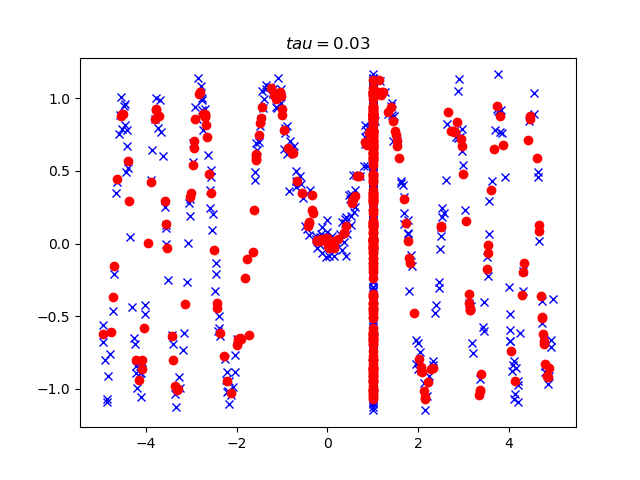
\includegraphics[width=\linewidth]{pics/tau_0d03}
    \end{subfigure}
    \begin{subfigure}[b]{0.5\linewidth}
        \centering
        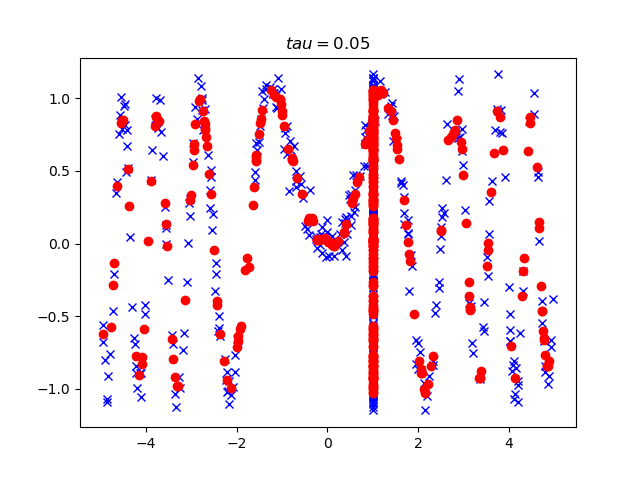
\includegraphics[width=\linewidth]{pics/tau_0d05}
    \end{subfigure}
    \begin{subfigure}[b]{0.5\linewidth}
        \centering
        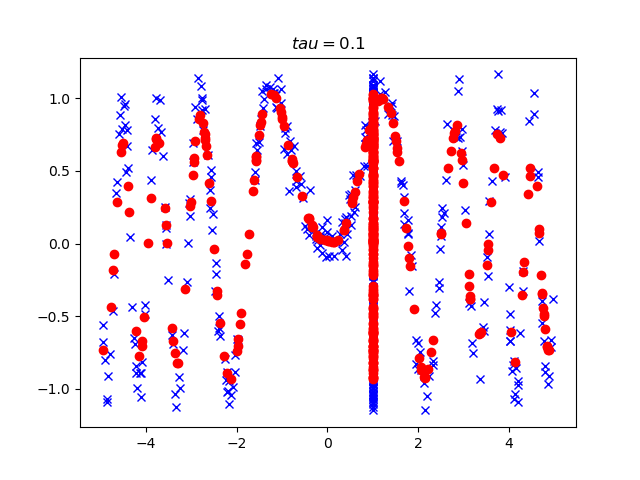
\includegraphics[width=\linewidth]{pics/tau_0d1}
    \end{subfigure}
    \begin{subfigure}[b]{0.5\linewidth}
        \centering
        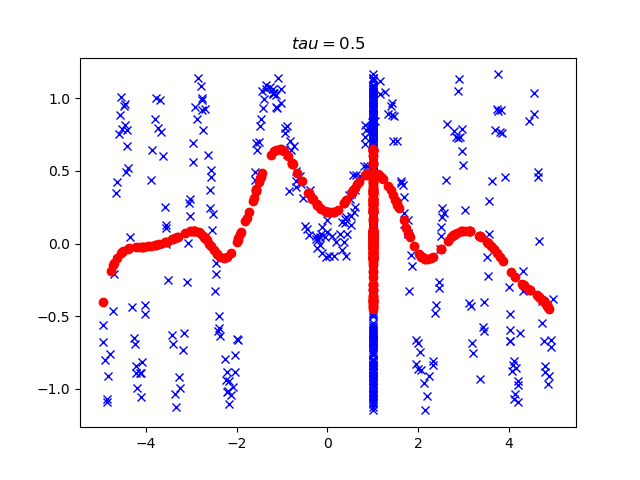
\includegraphics[width=\linewidth]{pics/tau_0d5}
    \end{subfigure}
    \begin{subfigure}[b]{0.5\linewidth}
        \centering
        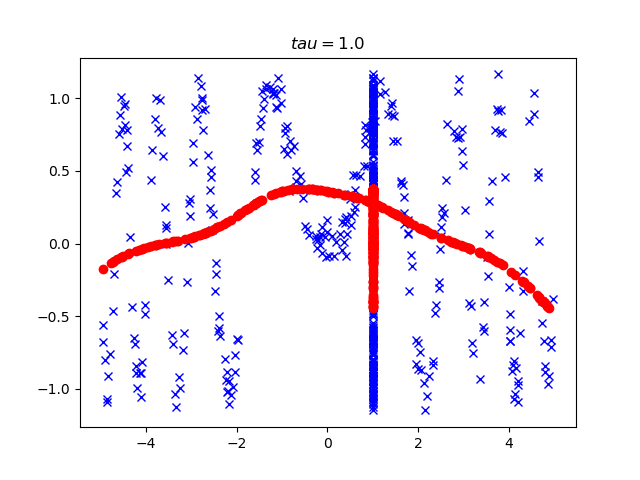
\includegraphics[width=\linewidth]{pics/tau_1d0}
    \end{subfigure}
    \begin{subfigure}[b]{0.5\linewidth}
        \centering
        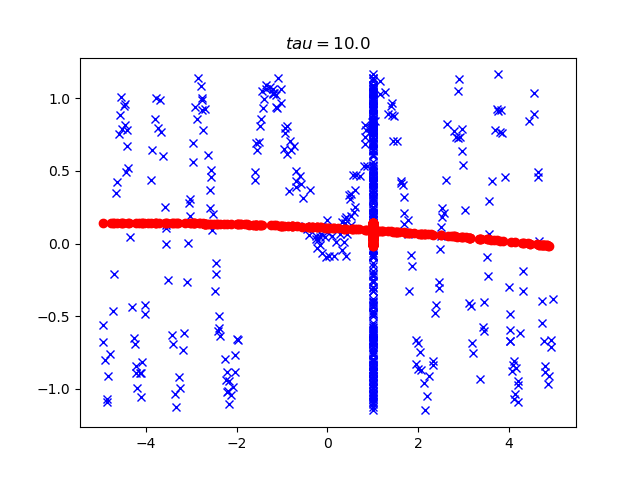
\includegraphics[width=\linewidth]{pics/tau_10d0}
    \end{subfigure}

$tau = 0.05$ achieve best result. MSE on valid set is $0.0124$, on test set is $0.0170$.

\end{figure}
\end{answer}

} \fi
